\cut{Thrust 1: A Foundation for Efficient Fuzzer Execution,
Orchestration, and Evaluation}


\jdh{Make it clear that 
1) big picture has user-provided compute resources, we aren't providing these for the world (fig caption and text body)
2) public outreach includes some free cloud time for early adopters to address point 1.
3) user-provided compute resources can be in a support cloud (OpenStack, Azure, AWS) or just a user multi-core machine via Vagrant/Docker
}


An infrastructure for (meta-)fuzzing research, 
whether for evaluating large sets of fuzzers in a (meta-)fuzzing approaches, 
evaluating architecture-specific fuzzing feature benefits, 
or for less-explored but promising research such as determining which kinds of 
fuzzers work best for broad classes of fuzzing, needs to be sufficiently 
efficient, robust and configurable to support a variety of (possibly 
unforeseen) requirements.  
Further, this infrastructure needs to be easily extendable to support new input 
mutators, benchmarks, input sharing, and new computation-providing backends 
(e.g., a new version of OpenStack.)

We propose an infrastructure, as shown in Figure~\ref{fig:overview} 
that meets these many various needs by focusing on 
simplicity and extensibility.  We propose an API based on:
on separating the needs of each component as thoroughly as possible.
For example, as the figure shows, input mutators are separated from the
individual fuzzer and each supported fuzzer will need to leverage the API to
mutate inputs.  Instrumentors (whether source or binary) will have to accept 
from the fuzzer a domain-specific language on how to instrument the program
and how to transform it for better fuzzing.  

Of particular note is the meta-fuzz coordinator server.
The coordinator leverages the specifications
of the compute resources to allocate compute containers (whether VMs, 
docker containers, or something else) that run an execution agent 
on the provisioned hardware.   The agent, running with elevated privileges, 
connects to the coordinator server to know what fuzzing actions to take.
The central server instructs agents to perform tasks such as 
installing software; starting fuzzing campaign with fuzzing parameters such as 
which mutator to use or how to exchange inputs; and post-campaign statistics to request.
The fuzzing-campaign director interacts with the meta-fuzz server to configure, start, 
monitor, interrupt, or gather statistics from a fuzzing campaign.  Further, a 
campaign director can upload a previously created configuration to the server 
to launch a campaign, allowing for repeatable operation and an easy mechanism to distribute
repeatable science to the CISE community.  

The figure shows a cloud providing compute resources for fuzzing campaigns.  
We leverage the meta-fuzzing infrastructure's API here such that "cloud" can 
mean practically anything the campaign director wants.  We definitely envision
supporting common cloud provider infrastructures such as OpenStack or CloudBank, but
also that a "cloud" can be as simple as the campaign-director's local, multi-core machine 
with Vagrant and Docker installed.  Optimizing easy development, experimentation and repeatability
of new techniques is key. 

To support these features, the infrastructure will come with pre-configured 
fuzzing campaigns, fuzzer configurations, input sharing schemas, and VM images to allow easy adoption for 
beginning users.  We plan to initially target Vagrant/Docker for single-machine operation, then OpenStack leveraging the UVA 
hardware resources available, as well as finally CloudBank AWS/Azure.

Lastly, we note that the infrastructure's configuration options will focus on general meta-fuzzing strategies 
to allow for easy user extensibility and CISE-supported extensions.  
End-users will be able to easily create 
new fuzzing components (e.g., input mutator, code instrumentation type, input 
sharing mechanisms) by writing new configuration files, schemas or 
pre-configured machine images.  The project will accept 
community-submitted extensions to our proposed open-source infrastructure when 
the project has achieved a initial acceptance and such opportunities become available.


\clg{TODO (for someone else): somewhere (here? In User Services? Who knows), need a
description of (a) initially supported fuzzers, and (b) interface for
adding/integrating new fuzzers.}

The following sections describe more detail about how meta-fuzzing can be realized 
in the proposed infrastructure.


\begin{figure}[htbp!]
% placeholder
%\vbox to 7in {\vfil
%\hbox to 7in{a figure to be drawn later}%
%\vfil
%}


% fbox to help visualizing trimming
%\fbox{
% Answer: [trim={left bottom right top},clip]
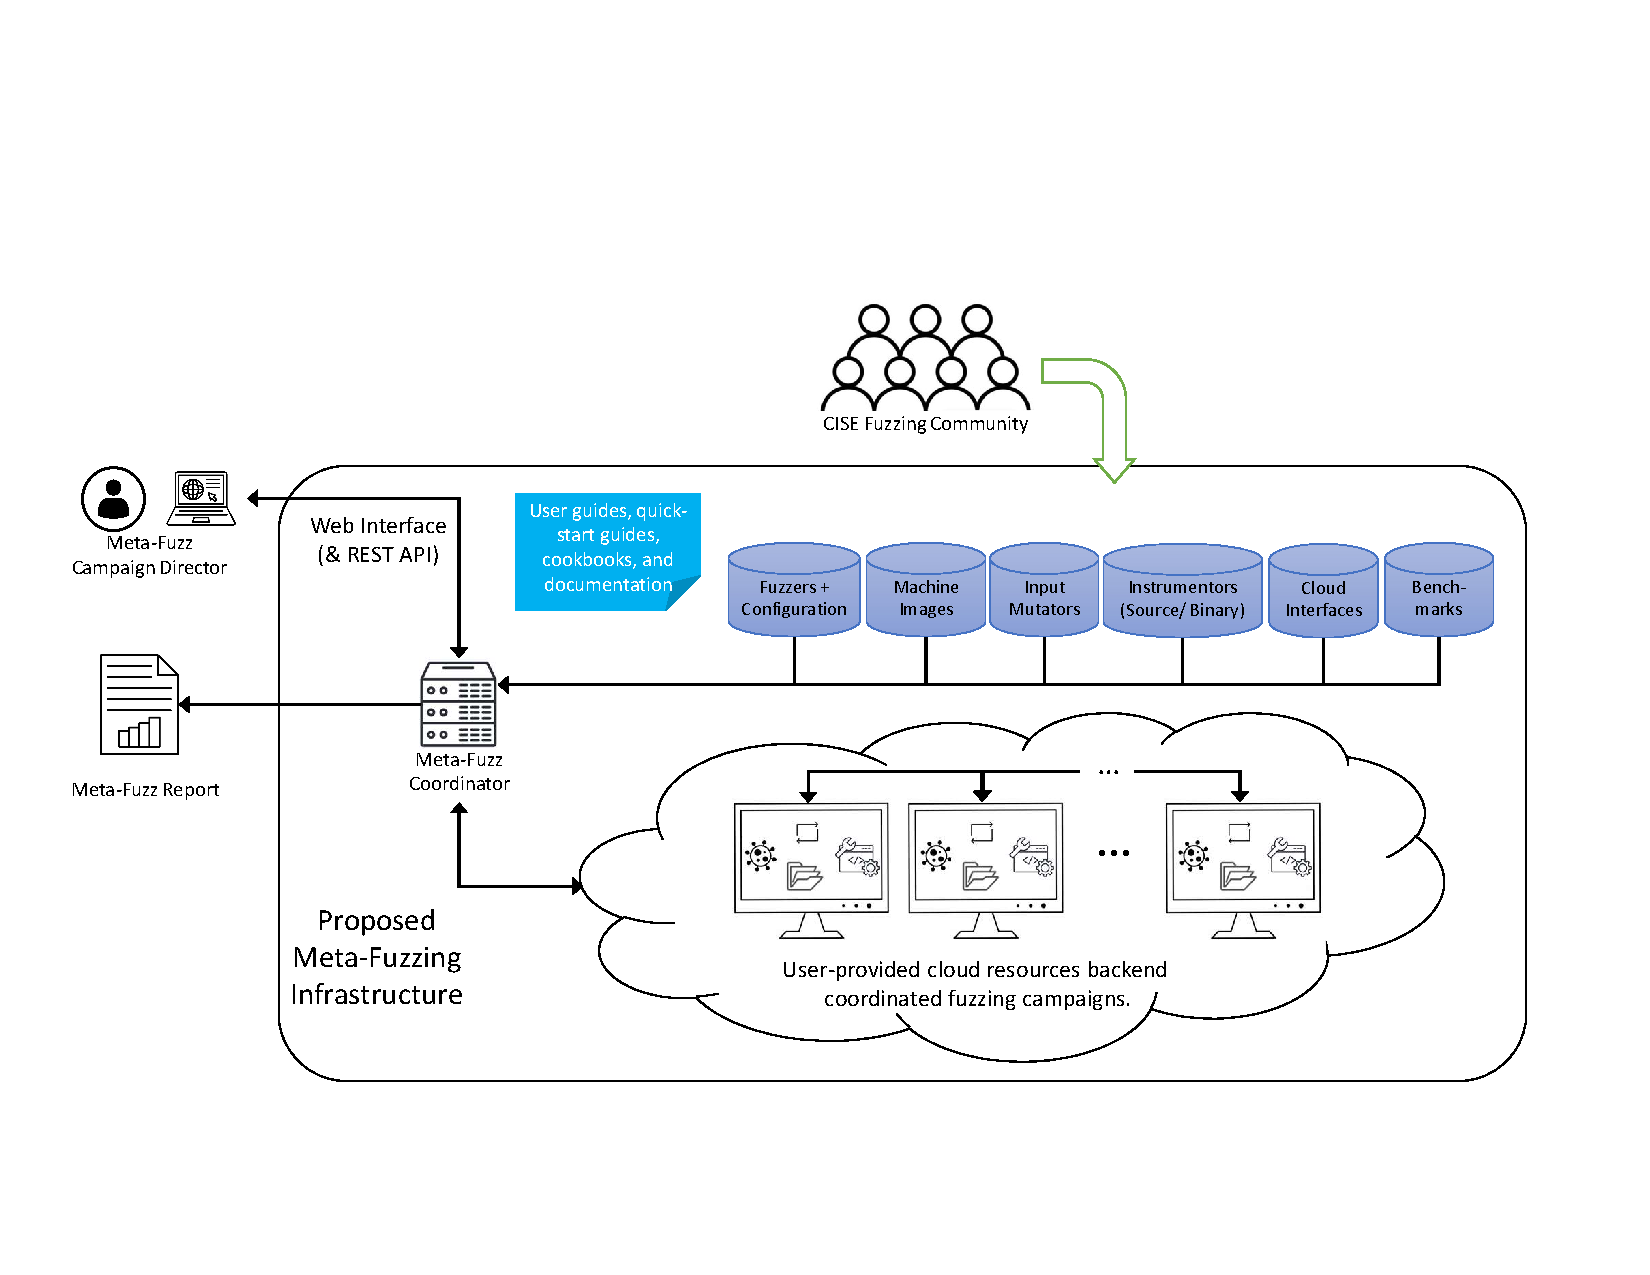
\includegraphics[width=\textwidth,trim={0.4in 1.25in 0.8in 2.0in},clip]{figures/mf-arch.pdf}
%}

\caption{Proposed Meta-fuzzing infrastructure overview.  
A fuzz-campaign director interacts with the meta-fuzzer server to setup or replay a configured fuzzing campaign.  
Built-in collections of of benchmarks, machine images, input sharing techniques, hardware resource requirements, input mutators, and other fuzzer configuration 
allow for quick startup of fuzzing campaigns backended by popular cloud service providers as well as configurability and extensibility for custom fuzzing setups.  
The system allows an experimenter to quickly and simply obtain results, or reproduce prior fuzzing campaigns.}
\label{fig:overview}
\end{figure}



\cut{

	\subsection{Thrust 1: A Foundation for Efficient Fuzzer Execution,
Orchestration, and Evaluation}

The execution of large sets of fuzzers for purposes of evaluating
(meta-)fuzzing approaches, or for less-explored but promising research such as
determining which kinds of fuzzers work best for broad classes of fuzzing
targets (e.g., compilers, media parsers, data structures, etc.) is essentially
the same core task as that required for sophisticated ensemble fuzzing.  The
only real difference is that a benchmarking run 1) runs all the fuzzers with
the same resource allocation and 2) there is no sharing of inputs between
fuzzers.  That is, fuzzer benchmarking is a simplified, restricted, version of
what is needed for a successful platform for implementing ensemble fuzzing.
The core needs are the same: ease of adding new fuzzers and including new
targets, ease of deployment to both local environments (for easy debugging or
use in developer ``unit fuzzing'') and the cloud (for large-scale fuzzing or
fuzzer evaluation), and ability to produce easily interpretable, statistically
usable, results (for both human consumption and resource allocation).

\jdh{UVA can you talk more about how to go about this thrust?}

fuzzers -- which fuzzers to use, and how to extend infrastructure for new 
fuzzers.  This is really NAU?
benchmarks -- standard fuzzing benchmarks, plus ability to add custom 
benchmarks.
specification -- which backend to use, how to allocate resources, how a fuzzing 
campaign should look like, which mutators to use, which instrumentation to use.
deployment -- VM allocation, software installation, efficient (semi-)automatic 
assignment of fuzzers based on fuzz campaign mapping
cooperation -- how often to share, and what to share.  Sharing "architectures" 
(e.g., share on the same VM, vs. different VMs in same cluster vs VMs in 
different clusters vs VMs in different data centers)
results -- collecting results (baseline results + user-specified extensions), 
statistical analysis


}
